% !TEX program = pdflatex
\documentclass[3p,11pt]{elsarticle}
\usepackage{amsmath,amssymb}
\usepackage{array}
\usepackage{booktabs}
\usepackage[tableposition=top]{caption}
\usepackage{enumitem}
\usepackage{tikz}
\usepackage{pgfplots}
\pgfplotsset{compat=1.18}
\usepackage{url}
\urlstyle{same}
\usepackage[hidelinks]{hyperref}
\emergencystretch=3em
% first-page footer: the page number alone
\makeatletter
\def\ps@pprintTitle{\let\@oddhead\@empty\let\@evenhead\@empty
  \def\@oddfoot{\hfil\thepage\hfil}\let\@evenfoot\@oddfoot}
\makeatother

% ---- notation ---------------------------------------------------------------
\newcommand{\um}{\,$\mu$m}
\newcommand{\kms}{km\,s$^{-1}$}
\newcommand{\flux}{erg\,cm$^{-2}$\,s$^{-1}$}
\newcommand{\mA}{m\AA}
\newcommand{\sci}[2]{#1\times10^{#2}}
\newcommand{\ion}[2]{#1\,\textsc{#2}}
\newcommand{\nuc}[2]{$^{#1}$#2}
\newcommand{\lxl}{$L_X/L_\mathrm{bol}$}

\begin{document}

\begin{frontmatter}

\title{A search for technetium, promethium and short-lived actinides in nearby Sun-like stars}

\author{Charles C. Norton}

\begin{abstract}
Technetium, promethium and the actinides from protactinium to curium have no isotope
that outlives a star, so their lines in a sun-like star would mean that atoms were added
to it recently, for instance as fission waste disposed of by a civilization. We search
$1413$ archival HARPS, UVES, FEROS and ESPRESSO spectra of $274$ F8 to K1 dwarfs within
$50$\,pc for absorption at $50$ lines of \ion{Tc}{i}, \ion{Pm}{ii}, \ion{Pa}{ii},
\ion{Pu}{ii}, \ion{Am}{ii} and \ion{Cm}{ii}. Each star's stacked spectrum is fitted at
each line by its six most similar stacks, and the element's combined absorption is
compared with the same measurement at $400$ random wavelengths of the same star. Of
$2262$ star-element tests, $9$ fall below $p=0.01$ where $22.6$ are expected, and each
of the nine takes its absorption from a stellar blend that other stars share or from a
feature wider than an unresolved line. The median limits on the equivalent width of an
element's strongest line run from $0.4$ to $5.3$\,m\AA, and lines injected at those
strengths are recovered at $p=0.0010$. With curves of growth from Korg, the HARPS and
ESPRESSO limits for solar-type stars are $A(\mathrm{Tc})<0.69$ and
$A(\mathrm{Pm})<-0.86$, near the solar abundance of thorium. Mixed through a solar
convective envelope, they amount to $\sci{1.7}{19}$\,kg of \nuc{99}{Tc} and
$\sci{7}{17}$\,kg of \nuc{147}{Pm}, the steady-state waste of $\sci{6}{21}$\,W and
$\sci{3.5}{25}$\,W of fission power; the technetium alone is the product of fissioning
$\sci{7}{20}$\,kg of \nuc{235}{U}, several thousand times the uranium of the Earth, so the
search constrains disposal on a scale far beyond a planet's fuel, as dilution through a
sun-like star's convective envelope requires.
\end{abstract}

\begin{keyword}
Technosignatures \sep Stars: abundances \sep Stars: solar-type \sep
Nuclear reactions, nucleosynthesis, abundances \sep Techniques: spectroscopic
\end{keyword}

\end{frontmatter}

% =============================================================================
\section{Introduction}\label{sec:intro}
% =============================================================================

Technetium, promethium and the actinides protactinium, plutonium, americium and curium
have no isotope that lasts the life of a star. The longest-lived isotopes decay in
$4.2$\,Myr (technetium), $17.7$\,yr (promethium), $33$\,kyr (protactinium), $81$\,Myr
(plutonium), $7.4$\,kyr (americium) and $16$\,Myr (curium), so a star a few billion
years old keeps none of the atoms of these elements it was born with, and their lines in
its spectrum mean the atoms were made or delivered recently. Merrill's detection of
technetium in S stars~\cite{Merrill1952} showed nucleosynthesis inside evolved stars,
but a main-sequence dwarf makes none of these elements.

That absence makes them a possible technosignature. Drake and Shklovskii suggested that
a civilization could announce itself by salting its star with a short-lived isotope, and
Sagan cautioned that normal and peculiar stellar spectra would have to be understood far
better before an unusual atom could be read as a sign of
intelligence~\cite{ShklovskiiSagan1966}. Whitmire and Wright proposed that a civilization
disposing of fission waste in its star would leave such lines without intending to, and
argued that convective dilution and stellar lifetimes favour stars of types A5 to
F2~\cite{WhitmireWright1980,Carrigan2010}. The only stars in which lines of these
elements have been reported are chemically peculiar: promethium in Przybylski's star
(HD~101065), HD~965 and HR~465~\cite{Cowley2004,Fivet2007}, and short-lived actinides
in Przybylski's star~\cite{Gopka2008}, where a synthesis of the \ion{Tc}{i}
$4297$\,\AA\ line limits technetium to $\log\epsilon(\mathrm{Tc})<2.5$~\cite{Andrievsky2023}
and a re-examination of three \ion{Pm}{ii} lines finds them too blended for
promethium to be claimed~\cite{Andrievsky2023b}.
Those reports remain disputed, since the spectra of such stars are crowded with lines of
the rare earths, and natural sources have been proposed, from nuclear reactions in the
atmosphere~\cite{Goriely2007} to the decay of long-lived superheavy
nuclei~\cite{Dzuba2017}.

The sun-like stars nearest the Sun, whose planets are the first targets of any search
for life, have not been searched for these elements. This paper does so with the
archival high-resolution spectra of the European Southern Observatory: we measure the
absorption at the lines of technetium, promethium, protactinium, plutonium, americium
and curium in the stacked spectra of nearby F8 to K1 dwarfs from four spectrographs,
compare it with the same measurement at random wavelengths of the same star, and turn
each star's sensitivity into an equivalent width, an abundance and a mass of material
mixed through the star's convective envelope.

\subsection{Contributions}
\begin{enumerate}[leftmargin=*,itemsep=1pt]
\item A search of $274$ nearby F8 to K1 dwarfs for six elements with no long-lived
isotope in $1413$ spectra from four spectrographs, with each star's limit on the
equivalent width, the abundance and the mass of each element.
\item A measurement against comparison stacks with a per-star empirical null, whose
limits follow from the measured line scores and are confirmed by injection.
\item Curves of growth of \ion{Tc}{i} and \ion{Pm}{ii} in dwarf atmospheres of
$5100$ to $6500$\,K, and the conversion of the limits into masses of fission products
and the fission power that would sustain them.
\end{enumerate}

% =============================================================================
\section{Data}\label{sec:data}
% =============================================================================

The spectra come from the ESO Science Archive and four spectrographs:
HARPS~\cite{Mayor2003}, UVES~\cite{Dekker2000}, FEROS~\cite{Kaufer1999} and
ESPRESSO~\cite{Pepe2021}. The UVES, FEROS and ESPRESSO samples are drawn from Gaia
DR3~\cite{Gaia2023}: every source with parallax above $20$\,mas,
$0.62<G_\mathrm{BP}-G_\mathrm{RP}<1.0$, $G<10$, a renormalised unit weight error below
$1.4$ and declination below $+30^\circ$, which selects the $1699$ single F8 to K1 dwarfs
within $50$\,pc that the southern telescopes reach~\cite{PecautMamajek2013}. For each
spectrograph we count the one-dimensional spectra within $30''$ of each star, take the
$150$ (UVES), $92$ (FEROS) and $94$ (ESPRESSO) nearest stars with at least two of them
and a Gaia radial velocity~\cite{Katz2023}, and download up to four spectra of each
covering $4220$--$4310$\,\AA, those of highest signal-to-noise ratio first. The HARPS
sample was drawn first and on narrower cuts: the $97$ stars within $30$\,pc with
$G<9$, declination below $+20^\circ$, the same colour and astrometric cuts, at least five
HARPS spectra, a Gaia radial velocity and fewer than $200$ references in SIMBAD ($8$ to
$194$), with up to six spectra each, highest signal-to-noise ratio first and one a night.
A file found within $30''$ of two stars, the members of a wide pair, belongs to the one
nearest the pointing in its header. Table~\ref{tab:data} lists the samples; together they
hold $1413$ spectra of $274$ distinct stars at $6.8$ to $47.3$\,pc (median $26.2$\,pc).

\begin{table}[t]
\centering\small
\caption{The samples. $R$ is the resolving power assumed for the matched filter, and
coverage the median span of a stack on the $4100$--$5600$\,\AA\ grid. Eligible stars are
those meeting the selection, of which the nearest are downloaded (all $97$ for HARPS),
with the number of spectra downloaded. Measured stars have a stack whose
best comparison stack correlates above $0.9$. S/N is the median signal-to-noise ratio
of a stack per $0.01$\,\AA\ sample at $4150$--$4550$\,\AA.}
\label{tab:data}
\begin{tabular}{l r c r r r r r}
\toprule
Spectrograph & $R$ & Coverage (\AA) & Eligible & Stars & Spectra & Measured & S/N \\
\midrule
HARPS & $115{,}000$ & $4100$--$5600$ & $97$ & $97$ & $582$ & $95$ & $72$ \\
UVES & $45{,}000$ & $4100$--$4524$ & $361$ & $150$ & $252$ & $116$ & $92$ \\
FEROS & $48{,}000$ & $4100$--$5600$ & $138$ & $92$ & $283$ & $80$ & $96$ \\
ESPRESSO & $140{,}000$ & $4100$--$5600$ & $102$ & $94$ & $296$ & $86$ & $63$ \\
\bottomrule
\end{tabular}
\end{table}

% =============================================================================
\section{Method}\label{sec:method}
% =============================================================================

\emph{Stacks.} Each spectrum is placed on a grid of $0.01$\,\AA\ from $4100$ to
$5600$\,\AA\ in air wavelengths and the barycentric frame, using the pipeline's frame
where the file declares one and otherwise a barycentric correction for the observatory at
mid-exposure. It is divided by its running upper envelope, the $92$nd percentile in
blocks of $3$\,\AA, and a star's spectra are median-stacked. A stack whose scatter
between adjacent samples exceeds $10$ per cent at $4150$--$4550$\,\AA\ is dropped. The
stack is moved to the star's rest frame by the velocity that puts the cores of up to
$30$ strong \ion{Fe}{i}, \ion{Ca}{i}, \ion{Mg}{i} and \ion{Ba}{ii} lines at their
laboratory wavelengths. These velocities follow the Gaia radial velocities with a robust
scatter of $0.11$\,\kms\ for HARPS and ESPRESSO, $0.25$\,\kms\ for FEROS and
$0.53$\,\kms\ for UVES, about median offsets of $+0.25$ to $+0.67$\,\kms. Nine stacks
differ from Gaia by more than $3$\,\kms: four are spectroscopic binaries or stars whose
Gaia velocities vary (HD~26491, $\tau^1$~Eri, AF~Lep and HD~189245), and five hold FEROS
spectra from 2003 December 7 and 8, whose reductions are offset by $4$ to $6$\,\kms.
Because each stack's frame comes from its own lines, neither affects the measurement.

\emph{Lines.} Table~\ref{tab:lines} lists the lines. Each line is weighted by its
expected strength in a $5800$\,K atmosphere, $\lambda^2 gf\exp(-E_\mathrm{low}/kT)$ for
the dominant ion, with the \ion{Tc}{i} oscillator strengths of Palmeri et
al.~\cite{Palmeri2005} and the \ion{Pm}{ii} values of Fivet et al.~\cite{Fivet2007}.
No oscillator strengths have been measured or computed for most lines of the singly
ionized actinides, so their relative intensities in the arc spectra compiled by
NIST~\cite{NIST} stand in for $gf$ and every lower level is taken as the ground. Arc
intensities depend on the source's excitation and on the detector as well as on $gf$,
so the actinide weights are uncertain by factors of a few, which shifts strength between
the lines of a combination but leaves each line's own measurement unchanged; the
actinide results are therefore reported as equivalent widths of the strongest line and
not as abundances. Lines
within $3$\,\AA\ of a Balmer line, and lines weaker than a tenth of the element's
strongest, are left out.

\begin{table}[t]
\centering\small
\caption{The lines measured and their weights relative to the element's strongest
line, $\lambda^2gf\exp(-E_\mathrm{low}/kT)$ at $5800$\,K. NIST lists all $23$
\ion{Pu}{ii} lines of the range at the same arc intensity.}
\label{tab:lines}
\begin{tabular}{l >{\raggedright\arraybackslash}p{0.62\textwidth} l}
\toprule
Ion & Air wavelengths (\AA) and weights & $gf$ \\
\midrule
\ion{Tc}{i} & 4238.19 (0.45), 4262.27 (0.71), 4297.06 (1.00) & Palmeri et al.~\cite{Palmeri2005} \\
\ion{Pm}{ii} & 4137.95 (0.59), 4157.86 (0.88), 4186.03 (1.00), 4297.78 (0.80), 4381.88 (0.12), 5546.08 (0.13), 5556.88 (0.11), 5561.73 (0.18), 5576.02 (0.20) & Fivet et al.~\cite{Fivet2007} \\
\ion{Pa}{ii} & 4217.23 (0.99), 4248.08 (1.00), 4176.18 (0.29), 4291.34 (0.31), 4601.43 (0.35) & NIST arc intensity \\
\ion{Pu}{ii} & 4105.95 (0.82), 4129.93 (0.83), 4141.20 (0.83), 4159.39 (0.84), 4178.28 (0.85), 4189.90 (0.85), 4190.06 (0.85), 4196.20 (0.86), 4229.77 (0.87), 4254.76 (0.88), 4273.34 (0.89), 4289.08 (0.89), 4337.18 (0.91), 4352.71 (0.92), 4379.91 (0.93), 4385.35 (0.93), 4393.93 (0.94), 4441.65 (0.96), 4468.54 (0.97), 4472.79 (0.97), 4493.78 (0.98), 4504.91 (0.99), 4536.15 (1.00) & NIST arc intensity \\
\ion{Am}{ii} & 4509.45 (0.97), 4575.59 (1.00), 4324.57 (0.36), 4441.36 (0.38), 4699.70 (0.42), 4872.22 (0.45), 4188.12 (0.17), 4593.31 (0.20), 5020.96 (0.24) & NIST arc intensity \\
\ion{Cm}{ii} & 4207.66 (1.00) & NIST arc intensity \\
\bottomrule
\end{tabular}
\end{table}

\emph{Measurement.} At each line we fit the $\pm8$\,\AA\ around it by a non-negative
combination of the six stacks of the same spectrograph that correlate best with the
star's, together with a signed linear continuum and signed first and second derivatives
of the fitted model, which absorb small differences of velocity and line width; the
$\pm0.25$\,\AA\ around the line is left out of the fit. A matched filter with the
spectrograph's Gaussian line profile, applied to the residual at the line, gives the
strength $z$ of any extra absorption in units of the residual's robust scatter and its
equivalent width. Stars whose best comparison stack correlates below $0.9$ are not
measured. The comparison stacks carry the star's own blends and the spectrograph's
artefacts, so the residual at a line is what the star has that stars like it lack.

\emph{Score and null.} An element's lines are combined into
$z_c=\sum_i w_iz_i/(\sum_i w_i^2)^{1/2}$, where $w_i$ are the weights. The same
measurement at $400$ random wavelengths of the same star, each at least $1$\,\AA\ from
any line of the six elements and from the Balmer lines and $10$\,\AA\ inside the
stack's coverage, as the lines measured are, is the null: $p$ is the fraction of
$20{,}000$ combinations of null values, drawn with the same weights, that fall at or
below $z_c$, and for a single line its rank among the null values. The null carries
whatever the comparison stacks fail to model at random places of the spectrum, and one
null per star serves all six elements. A line whose scores scatter across a
spectrograph's stars by more than $1.5$ times the median scatter of the stars' nulls
lies on a stellar feature that the comparison stacks do not follow and is left out of
that spectrograph's scores.

\emph{Limits.} A line injected into a stack is narrower than the part of the window left
out of the fit, since four standard deviations of the line profile span less than
$0.25$\,\AA\ for all four spectrographs, so it leaves the fitted model unchanged and
moves each $z_i$ in proportion to its equivalent width. A star's limit is therefore the
equivalent width of the element's strongest line, the others in proportion to their
weights, at which $z_c$ would have reached the $p=0.001$ point of the star's null, an
absorber removing a fraction of the light at its line in proportion to the stack's flux
there. For curium, whose one line gives a null of $400$ values, the limit places the
line at the most extreme of them. The limit follows from the measured line scores
without refitting, and injection checks it: lines of each element injected at the limit
into the stacks of twelve stars of each spectrograph, $288$ injections in all, are
recovered at a median $p$ of $0.0010$ for the elements with more than one line, with
$80$ per cent of them between $0.0008$ and $0.0013$.

\emph{Abundances.} We convert a limit into an abundance $A(\mathrm{X})=\log_{10}
(N_\mathrm{X}/N_\mathrm{H})+12$ with curves of growth computed by
Korg~\cite{Wheeler2023} in MARCS model atmospheres~\cite{Gustafsson2008} of solar
metallicity, from $5100$ to $6500$\,K with $\log g$ from $4.55$ to $4.35$, with hydrogen
lines left out of the synthesis so that Balmer wings do not enter the equivalent width.
A star's temperature comes from its $G_\mathrm{BP}-G_\mathrm{RP}$ colour through the dwarf
sequence of Pecaut and Mamajek~\cite{PecautMamajek2013}. A metallicity of $\pm0.3$\,dex
changes the \ion{Tc}{i} conversion by less than $0.01$\,dex and the \ion{Pm}{ii} one by
$0.09$\,dex. To turn an abundance into a mass we mix the element through a solar
convective envelope of $0.024\,M_\odot$ with a hydrogen mass fraction of
$0.74$~\cite{Bahcall2006}, and to turn the mass into a supply rate we hold it against
decay, which for fission products of \nuc{235}{U} at $200$\,MeV a fission and
cumulative yields of $6.13$ per cent (\nuc{99}{Tc}, half-life $\sci{2.111}{5}$\,yr) and
$2.23$ per cent (\nuc{147}{Pm}, $2.62$\,yr)~\cite{JEFF31} gives a fission power.

% =============================================================================
\section{Results}\label{sec:results}
% =============================================================================

\emph{No element departs from chance.} Table~\ref{tab:results} gives each element's
result in each spectrograph. Of the $2262$ star-element tests, $186$ fall below $p=0.1$,
$93$ below $0.05$, $9$ below $0.01$ and $1$ below $0.001$, where $226$, $113$, $22.6$ and
$2.3$ are expected; nine or fewer below $0.01$ has a Poisson probability of $0.001$. The
$p$ values gather toward the middle of their range and thin at both ends
(Figure~\ref{fig:pvals}), so the nulls, and the limits drawn from them, are
conservative. The scatter criterion makes them so: it leaves out the lines whose scores
spread most across a spectrograph's stars, $13$ to $19$ per cent of whose scores lie
beyond three times a star's robust null scatter, and the lines it keeps lie there in
$1.3$ to $2.8$ per cent of cases where the random wavelengths of the nulls do in $1.5$ to
$3.6$ per cent. The tests are not independent, since one null serves a star's six
elements. The lowest, $p=\sci{1.0}{-4}$ for americium in the G3~V star
HD~19467 (UVES), would be met by chance in $0.23$ of such sets of tests. Each of the nine
takes most of its absorption from one line. At eight of those lines at least six other
stars of the same spectrograph absorb at least half as deeply, the mark of a stellar
blend whose strength varies among stars: \ion{Am}{ii} $4324.57$\,\AA, which carries
HD~19467's score at $z=-19$, reaches below $z=-11$ in five other UVES stars. The ninth,
plutonium in the K1~V double star HD~7895 (HARPS, $p=0.0021$), absorbs across
$4536.10$--$4536.45$\,\AA, about $0.35$\,\AA\ and several times the width of an
unresolved line.

\begin{figure}[tp]
\centering
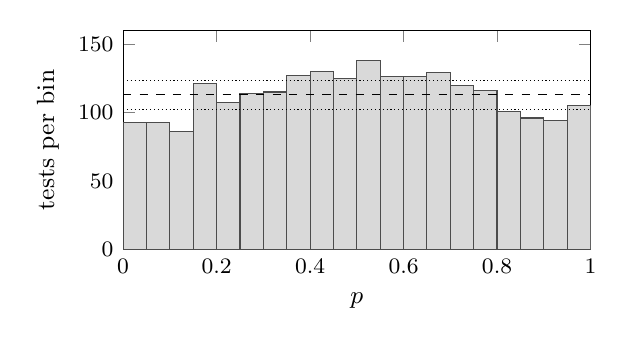
\begin{tikzpicture}
\begin{axis}[width=0.62\textwidth,height=0.36\textwidth,xmin=0,xmax=1,ymin=0,ymax=160,xlabel={$p$},ylabel={tests per bin},tick label style={font=\footnotesize},label style={font=\small},xtick={0,0.2,0.4,0.6,0.8,1},xticklabels={0,0.2,0.4,0.6,0.8,1}]
\addplot[ybar interval,fill=black!15,draw=black!70] coordinates {(0.00,93) (0.05,93) (0.10,86) (0.15,121) (0.20,107) (0.25,114) (0.30,115) (0.35,127) (0.40,130) (0.45,125) (0.50,138) (0.55,126) (0.60,126) (0.65,129) (0.70,120) (0.75,116) (0.80,101) (0.85,96) (0.90,94) (0.95,105) (1.00,105)};
\addplot[dashed,black,sharp plot] coordinates {(0,113.1) (1,113.1)};
\addplot[densely dotted,black,sharp plot] coordinates {(0,123.7) (1,123.7)};
\addplot[densely dotted,black,sharp plot] coordinates {(0,102.5) (1,102.5)};
\end{axis}
\end{tikzpicture}
\caption{The $p$ values of the $2262$ star-element tests in bins of $0.05$, against the
$113$ that a calibrated null puts in each bin (dashed) and its Poisson scatter
(dotted).}
\label{fig:pvals}
\end{figure}

\begin{table}[t]
\centering\small
\setlength{\tabcolsep}{4pt}
\caption{Results by element and spectrograph. $N$ is the number of stars measured,
$p_\mathrm{min}$ the lowest $p$ among them, and $W$ the median limit (m\AA) on the
equivalent width of the element's strongest line, the others in proportion to their
weights, at $p=0.001$ (for curium, beyond every value of the star's null).}
\label{tab:results}
\begin{tabular}{l rrr rrr rrr rrr}
\toprule
 & \multicolumn{3}{c}{HARPS} & \multicolumn{3}{c}{UVES} & \multicolumn{3}{c}{FEROS} & \multicolumn{3}{c}{ESPRESSO} \\
Ion & $N$ & $p_\mathrm{min}$ & $W$ & $N$ & $p_\mathrm{min}$ & $W$ & $N$ & $p_\mathrm{min}$ & $W$ & $N$ & $p_\mathrm{min}$ & $W$ \\
\midrule
\ion{Tc}{i} & $95$ & $0.038$ & $1.59$ & $116$ & $0.029$ & $3.80$ & $80$ & $0.061$ & $5.32$ & $86$ & $0.063$ & $1.60$ \\
\ion{Pm}{ii} & $95$ & $0.020$ & $0.94$ & $116$ & $0.029$ & $2.62$ & $80$ & $0.034$ & $3.35$ & $86$ & $0.019$ & $0.98$ \\
\ion{Pa}{ii} & $95$ & $0.016$ & $1.43$ & $116$ & $0.003$ & $2.87$ & $80$ & $0.017$ & $4.30$ & $86$ & $0.002$ & $1.30$ \\
\ion{Pu}{ii} & $95$ & $0.002$ & $0.42$ & $116$ & $0.005$ & $1.12$ & $80$ & $0.018$ & $1.26$ & $86$ & $0.030$ & $0.38$ \\
\ion{Am}{ii} & $95$ & $0.002$ & $0.57$ & $116$ & $0.0001$ & $3.40$ & $80$ & $0.013$ & $1.84$ & $86$ & $0.016$ & $0.53$ \\
\ion{Cm}{ii} & $95$ & $0.068$ & $1.72$ & $116$ & $0.017$ & $3.59$ & $80$ & $0.037$ & $5.30$ & $86$ & $0.087$ & $1.79$ \\
\bottomrule
\end{tabular}
\end{table}

\emph{Lines that follow the comparison stacks poorly.} Some plutonium lines lie on lines
of ionized metals, whose strength follows a star's gravity, metallicity and alpha
enhancement more closely than its comparison stacks do: \ion{Pu}{ii} $4468.54$\,\AA\ on
\ion{Ti}{ii} $4468.49$\,\AA\ and $4385.35$\,\AA\ on \ion{Fe}{ii} $4385.38$\,\AA. The
scatter criterion leaves out six \ion{Pu}{ii} lines in HARPS ($4254.76$, $4337.18$,
$4385.35$, $4393.93$, $4468.54$ and $4472.79$\,\AA), three in UVES and two each in
FEROS and ESPRESSO, and no line of the other elements. Without it, the $0.97$-weight
line at $4468.54$\,\AA\ alone gives Gaia DR3 5730371484020807808, a star moving at
$119$\,\kms, a plutonium score of $z=-17$ against its comparison stacks.

\emph{Limits.} The median limit on \ion{Tc}{i} $4297.06$\,\AA\ is $1.6$\,m\AA\ with
HARPS and ESPRESSO and $3.8$ and $5.3$\,m\AA\ with UVES and FEROS, whose resolving
powers are $2.4$ to $3$ times lower and whose UVES stacks mostly hold one spectrum. For
\ion{Pm}{ii} $4186.03$\,\AA\ the median limits are $0.9$ and $1.0$\,m\AA\ with HARPS and
ESPRESSO, and for plutonium, whose limit combines up to $21$ lines, $0.4$\,m\AA.
Figure~\ref{fig:abund} shows each star's technetium and promethium limit as an
abundance.

\begin{figure}[tp]
\centering
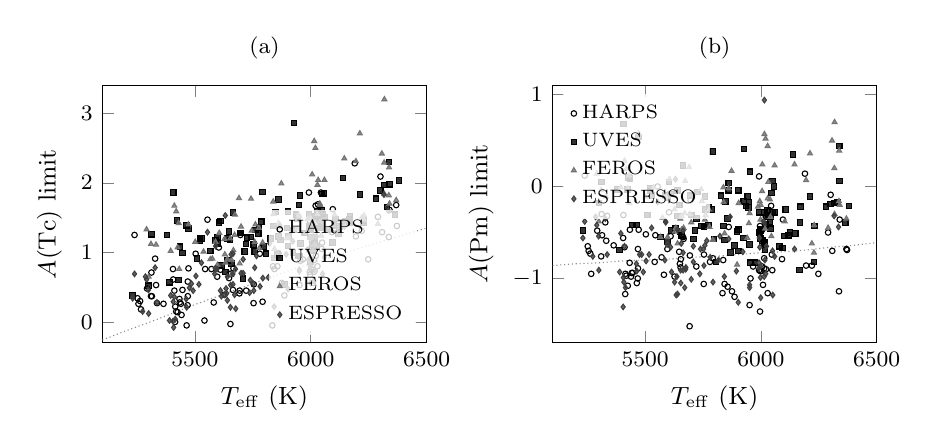
\begin{tikzpicture}
\begin{axis}[name=tc, width=0.47\textwidth,height=0.4\textwidth,xmin=5100,xmax=6500,ymin=-0.3,ymax=3.4,xlabel={$T_\mathrm{eff}$ (K)},ylabel={$A(\mathrm{Tc})$ limit},tick label style={font=\footnotesize},label style={font=\small},title={(a)},title style={font=\footnotesize},x tick label style={/pgf/number format/1000 sep={}},legend style={font=\scriptsize,at={(0.97,0.03)},anchor=south east,draw=none,fill=white,fill opacity=0.8,text opacity=1},legend cell align=left]
\addplot[only marks,mark=o,mark size=1.0pt,black,fill opacity=0.8] coordinates {(5239,1.25) (5252,0.34) (5256,0.26) (5263,0.30) (5267,0.18) (5293,0.48) (5310,0.37) (5312,0.71) (5314,0.37) (5328,0.91) (5332,0.53) (5336,0.27) (5364,0.26) (5405,0.76) (5406,0.61) (5411,0.45) (5414,-0.00) (5415,0.22) (5419,0.15) (5425,0.14) (5433,0.33) (5434,0.28) (5439,0.26) (5442,0.10) (5446,0.46) (5464,-0.05) (5468,0.24) (5469,0.37) (5469,0.58) (5472,0.77) (5503,0.98) (5541,0.02) (5544,0.76) (5554,1.47) (5571,0.76) (5581,0.28) (5596,0.65) (5603,1.07) (5610,0.75) (5627,0.39) (5647,0.63) (5650,0.69) (5653,-0.03) (5654,0.69) (5664,0.46) (5666,0.77) (5692,0.41) (5693,0.45) (5696,1.25) (5721,0.45) (5753,0.27) (5754,0.54) (5780,0.98) (5792,0.29) (5834,-0.05) (5837,0.80) (5843,0.76) (5856,0.80) (5861,0.99) (5875,0.56) (5886,0.38) (5951,0.53) (5955,0.88) (5966,0.90) (5992,1.86) (5992,1.04) (5996,0.72) (5996,1.45) (5997,0.68) (6003,0.76) (6005,0.75) (6006,1.49) (6009,0.56) (6014,0.72) (6014,0.89) (6021,1.67) (6022,0.95) (6029,0.80) (6031,1.69) (6044,1.86) (6047,1.05) (6049,1.14) (6091,1.29) (6095,1.62) (6190,2.28) (6195,1.23) (6220,1.31) (6248,0.90) (6290,1.51) (6301,2.09) (6308,1.29) (6337,1.22) (6340,1.61) (6369,1.68) (6372,1.38)};
\addlegendentry{HARPS}
\addplot[only marks,mark=square*,mark size=1.0pt,black,fill opacity=0.8] coordinates {(5231,0.38) (5300,0.52) (5312,1.26) (5379,1.25) (5390,0.57) (5406,1.86) (5423,1.46) (5429,0.60) (5435,1.08) (5446,0.99) (5464,1.39) (5472,1.34) (5509,0.91) (5521,1.17) (5522,1.20) (5529,1.20) (5566,1.02) (5589,1.17) (5597,1.22) (5598,1.13) (5603,1.43) (5610,1.45) (5614,0.81) (5632,0.72) (5640,1.20) (5640,0.88) (5647,1.30) (5652,1.18) (5658,0.84) (5664,1.57) (5696,1.28) (5699,1.28) (5708,0.62) (5715,1.01) (5721,1.12) (5725,1.21) (5742,1.22) (5754,1.11) (5758,1.01) (5761,1.32) (5773,1.27) (5776,1.36) (5786,1.44) (5792,1.87) (5797,1.08) (5806,0.98) (5827,1.20) (5839,1.38) (5843,0.92) (5848,1.58) (5855,0.97) (5861,1.76) (5861,1.23) (5869,1.18) (5886,0.54) (5897,1.35) (5902,1.59) (5902,1.09) (5904,1.23) (5924,1.00) (5926,1.32) (5927,2.86) (5936,1.54) (5943,1.49) (5946,0.95) (5949,1.68) (5951,0.95) (5953,1.82) (5955,1.13) (5974,1.28) (5992,1.55) (5992,1.37) (5996,1.32) (5997,1.22) (5998,0.86) (5999,1.39) (5999,1.33) (6006,1.11) (6014,1.03) (6014,1.43) (6015,1.16) (6017,1.21) (6020,1.52) (6024,1.08) (6029,1.59) (6030,1.53) (6039,1.35) (6041,1.46) (6044,1.36) (6046,1.61) (6049,1.84) (6050,1.55) (6057,1.85) (6060,1.50) (6079,1.33) (6094,1.14) (6101,1.39) (6107,1.48) (6120,1.27) (6125,1.37) (6139,2.07) (6148,1.45) (6166,1.43) (6168,1.47) (6170,1.52) (6212,1.83) (6229,1.42) (6230,1.46) (6281,1.77) (6300,1.89) (6318,1.97) (6330,1.65) (6338,2.30) (6340,1.98) (6364,1.54) (6381,2.03)};
\addlegendentry{UVES}
\addplot[only marks,mark=triangle*,mark size=1.0pt,black!55,fill opacity=0.8] coordinates {(5291,1.33) (5300,0.65) (5310,1.12) (5332,1.11) (5395,1.02) (5411,1.67) (5419,1.59) (5425,1.07) (5430,1.42) (5432,0.76) (5472,1.40) (5501,1.15) (5537,1.01) (5566,0.90) (5575,0.91) (5589,1.15) (5597,0.82) (5605,1.28) (5627,1.19) (5629,0.97) (5632,0.85) (5640,0.90) (5652,1.20) (5657,0.68) (5658,0.89) (5666,1.03) (5671,1.25) (5673,1.54) (5690,1.78) (5693,0.84) (5699,1.37) (5742,1.77) (5745,1.31) (5758,1.15) (5761,1.40) (5776,1.35) (5778,1.06) (5792,1.14) (5838,1.73) (5839,1.55) (5843,1.05) (5861,1.42) (5873,1.99) (5897,1.20) (5904,1.21) (5941,1.34) (5948,1.54) (5951,1.52) (5987,1.48) (5995,1.48) (5998,1.21) (5999,1.49) (6005,1.44) (6006,2.12) (6015,2.60) (6018,1.42) (6020,2.50) (6029,1.97) (6029,1.55) (6032,2.04) (6039,1.70) (6041,1.68) (6045,1.24) (6059,2.04) (6103,1.54) (6145,2.35) (6195,2.31) (6212,2.71) (6220,1.50) (6229,1.47) (6230,1.53) (6290,1.41) (6307,2.42) (6317,2.29) (6318,1.84) (6318,3.20) (6337,1.82) (6338,2.22) (6340,1.70) (6369,1.75)};
\addlegendentry{FEROS}
\addplot[only marks,mark=diamond*,mark size=1.0pt,black!75,fill opacity=0.8] coordinates {(5231,0.34) (5239,0.69) (5274,0.15) (5286,0.65) (5291,0.61) (5299,0.46) (5300,0.12) (5328,0.78) (5336,0.28) (5390,0.02) (5395,0.38) (5405,0.01) (5406,0.29) (5408,-0.08) (5411,0.36) (5415,0.04) (5462,0.33) (5464,0.21) (5476,0.49) (5485,0.55) (5492,0.45) (5504,0.66) (5517,0.54) (5528,0.85) (5554,1.29) (5585,0.69) (5588,0.77) (5589,1.09) (5595,0.76) (5610,0.45) (5614,0.37) (5627,0.39) (5631,1.53) (5634,0.48) (5637,0.41) (5640,0.31) (5640,0.65) (5653,0.21) (5654,0.53) (5656,0.97) (5664,0.98) (5664,0.69) (5664,0.54) (5671,0.39) (5675,0.76) (5676,0.19) (5699,0.70) (5708,0.70) (5708,0.90) (5736,0.42) (5739,0.60) (5752,0.55) (5754,0.45) (5758,0.78) (5766,0.95) (5781,0.51) (5793,0.63) (5817,0.64) (5823,1.13) (5842,0.22) (5861,1.22) (5867,1.38) (5894,0.97) (5902,0.47) (5922,1.16) (5951,0.73) (5951,0.75) (5991,0.89) (5992,0.90) (5993,1.02) (5995,1.21) (5998,0.80) (5998,0.80) (5999,0.56) (6011,1.23) (6014,0.59) (6015,3.50) (6017,1.11) (6021,0.73) (6024,1.23) (6050,1.45) (6051,0.69) (6059,0.93) (6145,1.37) (6316,1.83) (6335,1.60)};
\addlegendentry{ESPRESSO}
\addplot[densely dotted,black!45,forget plot] coordinates {(5100,-0.26) (5200,-0.13) (5300,-0.01) (5400,0.12) (5500,0.25) (5600,0.37) (5700,0.49) (5800,0.61) (5900,0.73) (6000,0.84) (6100,0.94) (6200,1.05) (6300,1.15) (6400,1.25) (6500,1.35)};
\end{axis}
\begin{axis}[at={(tc.east)},anchor=west,xshift=1.6cm, width=0.47\textwidth,height=0.4\textwidth,xmin=5100,xmax=6500,ymin=-1.7,ymax=1.1,xlabel={$T_\mathrm{eff}$ (K)},ylabel={$A(\mathrm{Pm})$ limit},tick label style={font=\footnotesize},label style={font=\small},title={(b)},title style={font=\footnotesize},x tick label style={/pgf/number format/1000 sep={}},legend style={font=\scriptsize,at={(0.03,0.97)},anchor=north west,draw=none,fill=white,fill opacity=0.8,text opacity=1},legend cell align=left]
\addplot[only marks,mark=o,mark size=1.0pt,black,fill opacity=0.8] coordinates {(5239,0.12) (5252,-0.65) (5256,-0.70) (5263,-0.73) (5267,-0.95) (5293,-0.48) (5310,-0.76) (5312,-0.30) (5314,-0.53) (5328,-0.39) (5332,-0.59) (5336,-0.32) (5364,-0.64) (5405,-0.56) (5406,-0.31) (5411,-0.66) (5414,-1.17) (5415,-0.95) (5419,-0.97) (5425,-1.08) (5433,-0.83) (5434,-0.47) (5439,-0.98) (5442,-0.94) (5446,-0.94) (5464,-1.05) (5468,-1.00) (5469,-0.89) (5469,-0.68) (5472,-0.47) (5503,-0.52) (5541,-0.82) (5544,-0.53) (5554,0.00) (5571,-0.77) (5581,-0.96) (5596,-0.68) (5603,-0.28) (5610,-0.54) (5627,-0.98) (5647,-0.71) (5650,-0.84) (5653,-0.88) (5654,-0.79) (5664,-0.55) (5666,-0.57) (5692,-1.52) (5693,-0.75) (5696,-0.15) (5721,-0.87) (5753,-1.06) (5754,-0.74) (5780,-0.82) (5792,-0.78) (5834,-1.16) (5837,-0.80) (5843,-1.06) (5856,-1.09) (5861,-0.44) (5875,-1.14) (5886,-1.20) (5951,-1.29) (5955,-1.00) (5966,-0.87) (5992,0.11) (5992,-0.91) (5996,-1.36) (5996,-0.43) (5997,-0.92) (6003,-0.92) (6005,-0.87) (6006,-0.47) (6009,-1.07) (6014,-0.89) (6014,-0.78) (6021,-0.33) (6022,-0.90) (6029,-1.16) (6031,-0.27) (6044,-0.21) (6047,-0.74) (6049,-0.91) (6091,-0.79) (6095,-0.36) (6190,0.14) (6195,-0.86) (6220,-0.86) (6248,-0.95) (6290,-0.50) (6301,-0.09) (6308,-0.70) (6337,-1.14) (6340,-0.36) (6369,-0.68) (6372,-0.69)};
\addlegendentry{HARPS}
\addplot[only marks,mark=square*,mark size=1.0pt,black,fill opacity=0.8] coordinates {(5231,-0.48) (5300,-0.18) (5312,0.05) (5379,-0.03) (5390,-0.69) (5406,0.68) (5423,-0.03) (5429,0.10) (5435,0.09) (5446,-0.42) (5464,-0.42) (5472,0.54) (5509,-0.31) (5521,-0.02) (5522,-0.05) (5529,-0.10) (5566,-0.55) (5589,-0.10) (5597,-0.60) (5598,-0.12) (5603,0.05) (5610,-0.08) (5614,-0.48) (5632,-0.45) (5640,-0.04) (5640,-0.32) (5647,-0.20) (5652,-0.49) (5658,-0.53) (5664,0.23) (5696,-0.10) (5699,-0.31) (5708,-0.57) (5715,-0.48) (5721,-0.35) (5725,-0.06) (5742,-0.43) (5754,-0.44) (5758,-0.11) (5761,-0.25) (5773,-0.42) (5776,-0.23) (5786,-0.25) (5792,0.38) (5797,-0.57) (5806,-0.82) (5827,-0.10) (5839,-0.43) (5843,-0.58) (5848,-0.16) (5855,-0.35) (5861,0.04) (5861,-0.04) (5869,-0.72) (5886,-0.64) (5897,-0.49) (5902,-0.04) (5902,-0.70) (5904,-0.47) (5924,-0.56) (5926,-0.16) (5927,0.41) (5936,-0.21) (5943,-0.11) (5946,-0.23) (5949,-0.17) (5951,-0.63) (5953,0.16) (5955,-0.83) (5974,-0.83) (5992,-0.28) (5992,-0.50) (5996,-0.50) (5997,-0.57) (5998,-0.47) (5999,-0.48) (5999,-0.56) (6006,-0.59) (6014,-0.61) (6014,-0.28) (6015,-0.62) (6017,-0.69) (6020,-0.41) (6024,-0.33) (6029,-0.26) (6030,-0.31) (6039,-0.38) (6041,-0.46) (6044,-0.33) (6046,-0.07) (6049,0.06) (6050,-0.28) (6057,0.00) (6060,-0.28) (6079,-0.65) (6094,-0.67) (6101,-0.54) (6107,-0.25) (6120,-0.53) (6125,-0.50) (6139,0.35) (6148,-0.51) (6166,-0.91) (6168,-0.39) (6170,-0.22) (6212,-0.11) (6229,-0.82) (6230,-0.43) (6281,-0.22) (6300,-0.19) (6318,-0.18) (6330,-0.17) (6338,0.44) (6340,0.06) (6364,-0.39) (6381,-0.21)};
\addlegendentry{UVES}
\addplot[only marks,mark=triangle*,mark size=1.0pt,black!55,fill opacity=0.8] coordinates {(5291,0.14) (5300,-0.38) (5310,-0.04) (5332,-0.11) (5395,-0.01) (5411,0.28) (5419,0.19) (5425,-0.02) (5430,0.12) (5432,-0.18) (5472,0.58) (5501,-0.11) (5537,-0.01) (5566,-0.55) (5575,-0.34) (5589,-0.11) (5597,-0.55) (5605,0.08) (5627,-0.25) (5629,-0.49) (5632,-0.45) (5640,-0.62) (5652,-0.35) (5657,-0.47) (5658,-0.32) (5666,-0.45) (5671,-0.29) (5673,0.06) (5690,0.21) (5693,-0.30) (5699,-0.39) (5742,-0.03) (5745,-0.16) (5758,-0.36) (5761,-0.31) (5776,-0.25) (5778,-0.44) (5792,-0.58) (5838,-0.01) (5839,-0.17) (5843,-0.51) (5861,-0.02) (5873,0.17) (5897,-0.85) (5904,-0.18) (5941,-0.56) (5948,-0.40) (5951,-0.29) (5987,-0.22) (5995,-0.16) (5998,-0.36) (5999,-0.20) (6005,-0.05) (6006,0.24) (6015,0.57) (6018,-0.46) (6020,0.52) (6029,0.44) (6029,-0.13) (6032,0.05) (6039,-0.14) (6041,-0.33) (6045,-0.54) (6059,0.23) (6103,-0.38) (6145,0.24) (6195,0.07) (6212,0.36) (6220,-0.62) (6229,-0.72) (6230,-0.42) (6290,-0.45) (6307,0.50) (6317,0.20) (6318,-0.30) (6318,0.70) (6337,-0.16) (6338,0.39) (6340,-0.20) (6369,-0.35)};
\addlegendentry{FEROS}
\addplot[only marks,mark=diamond*,mark size=1.0pt,black!75,fill opacity=0.8] coordinates {(5231,-0.56) (5239,-0.38) (5274,-0.76) (5286,-0.33) (5291,-0.42) (5299,-0.54) (5300,-0.91) (5328,-0.35) (5336,-0.74) (5390,-0.93) (5395,-0.51) (5405,-1.31) (5406,-0.99) (5408,-1.04) (5411,-0.65) (5415,-1.10) (5462,-0.84) (5464,-0.92) (5476,-0.74) (5485,-0.74) (5492,-0.93) (5504,-0.81) (5517,-0.74) (5528,-0.45) (5554,-0.17) (5585,-0.80) (5588,-0.38) (5589,-0.39) (5595,-0.63) (5610,-0.66) (5614,-0.93) (5627,-1.04) (5631,0.08) (5634,-1.18) (5637,-0.98) (5640,-1.17) (5640,-0.47) (5653,-0.91) (5654,-1.05) (5656,-0.62) (5664,-0.48) (5664,-0.91) (5664,-0.72) (5671,-1.10) (5675,-0.90) (5676,-0.88) (5699,-1.01) (5708,-0.82) (5708,-0.65) (5736,-0.95) (5739,-0.68) (5752,-0.68) (5754,-0.86) (5758,-0.64) (5766,-0.59) (5781,-0.77) (5793,-1.04) (5817,-0.80) (5823,-0.54) (5842,-0.98) (5861,-0.57) (5867,-0.33) (5894,-0.92) (5902,-1.26) (5922,-0.71) (5951,-1.07) (5951,-1.10) (5991,-0.89) (5992,-0.83) (5993,-0.56) (5995,-0.66) (5998,-0.99) (5998,-0.87) (5999,-1.21) (6011,-0.38) (6014,-0.98) (6015,0.94) (6017,-0.80) (6021,-0.95) (6024,-0.65) (6050,-0.70) (6051,-1.18) (6059,-0.76) (6145,-0.68) (6316,-0.32) (6335,-0.44)};
\addlegendentry{ESPRESSO}
\addplot[densely dotted,black!45,forget plot] coordinates {(5100,-0.86) (5200,-0.84) (5300,-0.83) (5400,-0.81) (5500,-0.80) (5600,-0.79) (5700,-0.77) (5800,-0.76) (5900,-0.74) (6000,-0.72) (6100,-0.71) (6200,-0.69) (6300,-0.66) (6400,-0.64) (6500,-0.61)};
\end{axis}
\end{tikzpicture}
\caption{Each star's abundance limit against its temperature: (a)~technetium from \ion{Tc}{i} $4297.06$\,\AA\ and (b)~promethium from \ion{Pm}{ii} $4186.03$\,\AA. The dotted curves mark the abundance at which the line's equivalent width is $1$\,m\AA. The curves of growth run from $A=-1$ to $3.5$; one FEROS technetium limit lies above the top of that grid and is drawn at it.}
\label{fig:abund}
\end{figure}

\emph{Abundances, masses and power.} \ion{Tc}{i} is a minority species whose ionization
rises steeply with temperature, so $1$\,m\AA\ in the $4297$\,\AA\ line corresponds to
$A(\mathrm{Tc})=-0.13$ at $5200$\,K, $0.61$ at $5800$\,K and $1.25$ at $6400$\,K, while
the same equivalent width in \ion{Pm}{ii} $4186$\,\AA, the dominant ion, corresponds to
$A(\mathrm{Pm})$ between $-0.84$ and $-0.64$ across that range. The median limits are
$A(\mathrm{Tc})<0.72$ and $0.66$ with HARPS and ESPRESSO and $1.32$ and $1.42$ with UVES
and FEROS, and the deepest is $-0.08$; for promethium they are $-0.78$, $-0.76$,
$-0.31$ and $-0.18$, and the deepest $-1.52$. These are near the solar abundance of
thorium, $A(\mathrm{Th})=0.02$~\cite{Asplund2009}, and two dex below the technetium limit
in Przybylski's star~\cite{Andrievsky2023}. For the HARPS and ESPRESSO stars of
$5600$ to $6000$\,K, the median limits $A(\mathrm{Tc})<0.69$ and $A(\mathrm{Pm})<-0.86$
correspond to $\sci{1.7}{19}$\,kg of \nuc{99}{Tc} and $\sci{7}{17}$\,kg of
\nuc{147}{Pm} in a solar convective envelope. Holding them there against decay takes
$\sci{5.6}{13}$\,kg of technetium or $\sci{1.9}{17}$\,kg of promethium a year, the
products of fissioning \nuc{235}{U} at $\sci{5.6}{21}$\,W or $\sci{3.5}{25}$\,W, which
is $0.09$ of the Sun's luminosity. Put as fuel rather than power, $\sci{1.7}{19}$\,kg of
\nuc{99}{Tc} at a cumulative yield of $6.1$ per cent is the product of $\sci{1.7}{45}$
fissions, $\sci{6.6}{20}$\,kg of \nuc{235}{U}, where the Earth's mantle and crust hold
about $\sci{8}{16}$\,kg of uranium of all isotopes~\cite{McDonough1995} and
$\sci{6}{14}$\,kg of \nuc{235}{U}: the limit lies three to six orders of magnitude above
what fissioning a planet's uranium could put into its star, and the \ion{Pm}{ii} limit,
set by a $2.6$\,yr half-life, correspondingly higher as a rate.

% =============================================================================
\section{Related work}\label{sec:related}
% =============================================================================

\emph{Technosignatures in stellar composition.} The proposals of Drake and
Shklovskii~\cite{ShklovskiiSagan1966} and of Whitmire and Wright~\cite{WhitmireWright1980}
are reviewed with other signatures of interstellar archaeology by
Carrigan~\cite{Carrigan2010}; we find no earlier search of ordinary dwarfs for the
elements they name.

\emph{Short-lived elements in stars.} Technetium is the signature of the third dredge-up
in asymptotic giant branch stars, and its presence or absence separates S stars that
make their own s-process elements from those that received them from a
companion~\cite{Merrill1952,VanEckJorissen1999}. Promethium and the short-lived actinides
have been reported only in the chemically peculiar Ap stars Przybylski's star, HD~965 and
HR~465~\cite{Cowley2004,Fivet2007,Gopka2008}, whose strong magnetic fields and
stratified atmospheres concentrate the rare earths in the layers that form their spectra;
in Przybylski's star itself technetium is limited to
$\log\epsilon(\mathrm{Tc})<2.5$~\cite{Andrievsky2023}.

\emph{Surveys of nearby stars.} The archival spectra used here were taken to measure
radial velocities and abundances, and the abundance surveys built on them report the
elements whose lines are strong in sun-like stars; none reports technetium, promethium
or the actinides beyond thorium.

% =============================================================================
\section{Conclusion}\label{sec:conclusion}
% =============================================================================

No line of technetium, promethium, protactinium, plutonium, americium or curium is found
in the archival HARPS, UVES, FEROS and ESPRESSO spectra of $274$ sun-like stars within
$50$\,pc. Every low $p$ has its absorption from a stellar blend that other stars share or
from a feature wider than an unresolved line, and the limits reach abundances near the
Sun's thorium abundance in the best spectra.

The limits apply to atoms in the photosphere at the epochs of the archival spectra, and
the conversion into masses assumes the element mixed through a convective envelope as
massive as the Sun's; a star's own envelope, thinner in F stars and thicker in K stars, scales the
mass in proportion. In a sun-like star the envelope's mass turns small abundances into
masses that no planetary industry reaches: the technetium limit is the waste of several
thousand Earths' worth of uranium, so what the search excludes is disposal on the scale
of a civilization that mines its whole planetary system, or that fissions its star's own
uranium, sustained for longer than the products' half-lives. That is the dilution
Whitmire and Wright foresaw, and the stars they preferred, A5 to F2 dwarfs whose thin
envelopes dilute a thousand times less, are not in the sample, nor are the Ap stars in
which diffusion concentrates heavy elements in the photosphere; both have archival
spectra from the same spectrographs, and the same measurement applied to them is where
a planetary-scale signal could be found.

\section*{Acknowledgements}

This work is based on observations collected at the European Southern Observatory and
obtained from the ESO Science Archive Facility. It has made use of data from the
European Space Agency mission Gaia, processed by the Gaia Data Processing and Analysis
Consortium (DPAC), funded by national institutions, in particular those participating
in the Gaia Multilateral Agreement. It uses the NIST Atomic Spectra
Database~\cite{NIST}, the spectral synthesis code Korg~\cite{Wheeler2023} with MARCS
model atmospheres~\cite{Gustafsson2008}, and the software Astropy~\cite{Astropy2022},
NumPy~\cite{Harris2020} and SciPy~\cite{Virtanen2020}.

\begin{thebibliography}{99}\small\raggedright
\setlength{\itemsep}{1pt}

\bibitem{Merrill1952}
P.~W. Merrill, Spectroscopic observations of stars of class S, \emph{Astrophys. J.}
\textbf{116}, 21 (1952).

\bibitem{ShklovskiiSagan1966}
I.~S. Shklovskii and C.~Sagan, \emph{Intelligent Life in the Universe} (Holden-Day, San
Francisco, 1966).

\bibitem{WhitmireWright1980}
D.~P. Whitmire and D.~P. Wright, Nuclear waste spectrum as evidence of technological
extraterrestrial civilizations, \emph{Icarus} \textbf{42}, 149 (1980).

\bibitem{Carrigan2010}
R.~A. Carrigan, Starry messages: searching for signatures of interstellar archaeology,
arXiv:1001.5455 (2010).

\bibitem{Cowley2004}
C.~R. Cowley, W.~P. Bidelman, S.~Hubrig, G.~Mathys and D.~J. Bord, On the possible
presence of promethium in the spectra of HD~101065 (Przybylski's star) and HD~965,
\emph{Astron. Astrophys.} \textbf{419}, 1087 (2004).

\bibitem{Fivet2007}
V.~Fivet, P.~Quinet, \'E.~Bi\'emont, A.~Jorissen, A.~V. Yushchenko and S.~Van~Eck,
Transition probabilities in singly ionized promethium and the identification of
\ion{Pm}{ii} lines in Przybylski's star and HR~465, \emph{Mon. Not. R. Astron. Soc.}
\textbf{380}, 771 (2007).

\bibitem{Gopka2008}
V.~F. Gopka, A.~V. Yushchenko, V.~A. Yushchenko, I.~V. Panov and Ch.~Kim,
Identification of absorption lines of short half-life actinides in the spectrum of
Przybylski's star (HD~101065), \emph{Kinemat. Phys. Celest. Bodies} \textbf{24}, 89
(2008).

\bibitem{Andrievsky2023}
S.~M. Andrievsky, S.~A. Korotin and K.~Werner, Abundance of radioactive technetium in
Przybylski's star revisited, \emph{Astron. Nachr.} \textbf{344}, e230077 (2023).

\bibitem{Andrievsky2023b}
S.~M. Andrievsky, S.~A. Korotin, K.~Werner and V.~V. Kovtyukh, An enigma of
Przybylski's star: is there promethium on its surface?, \emph{Astron. Nachr.}
\textbf{344}, e230056 (2023).

\bibitem{McDonough1995}
W.~F. McDonough and S.-s. Sun, The composition of the Earth, \emph{Chem. Geol.}
\textbf{120}, 223 (1995).

\bibitem{Goriely2007}
S.~Goriely, Nucleosynthesis by accelerated particles to account for the surface
composition of HD~101065, \emph{Astron. Astrophys.} \textbf{466}, 619 (2007).

\bibitem{Dzuba2017}
V.~A. Dzuba, V.~V. Flambaum and J.~K. Webb, Isotope shift and search for metastable
superheavy elements in astrophysical data, \emph{Phys. Rev. A} \textbf{95}, 062515
(2017).

\bibitem{VanEckJorissen1999}
S.~Van~Eck and A.~Jorissen, The Henize sample of S stars. I. The technetium dichotomy,
\emph{Astron. Astrophys.} \textbf{345}, 127 (1999).

\bibitem{Gaia2023}
Gaia Collaboration, A.~Vallenari, A.~G.~A. Brown, et al., Gaia Data Release 3: summary
of the content and survey properties, \emph{Astron. Astrophys.} \textbf{674}, A1 (2023).

\bibitem{Katz2023}
D.~Katz, P.~Sartoretti, A.~Guerrier, et al., Gaia Data Release 3: properties and
validation of the radial velocities, \emph{Astron. Astrophys.} \textbf{674}, A5 (2023).

\bibitem{PecautMamajek2013}
M.~J. Pecaut and E.~E. Mamajek, Intrinsic colors, temperatures, and bolometric
corrections of pre-main-sequence stars, \emph{Astrophys. J. Suppl.} \textbf{208}, 9
(2013).

\bibitem{Mayor2003}
M.~Mayor, F.~Pepe, D.~Queloz, et al., Setting new standards with HARPS, \emph{The
Messenger} \textbf{114}, 20 (2003).

\bibitem{Dekker2000}
H.~Dekker, S.~D'Odorico, A.~Kaufer, B.~Delabre and H.~Kotzlowski, Design, construction,
and performance of UVES, the echelle spectrograph for the UT2 Kueyen Telescope at the
ESO Paranal Observatory, \emph{Proc. SPIE} \textbf{4008}, 534 (2000).

\bibitem{Kaufer1999}
A.~Kaufer, O.~Stahl, S.~Tubbesing, et al., Commissioning FEROS, the new high-resolution
spectrograph at La Silla, \emph{The Messenger} \textbf{95}, 8 (1999).

\bibitem{Pepe2021}
F.~Pepe, S.~Cristiani, R.~Rebolo, et al., ESPRESSO at VLT: on-sky performance and first
results, \emph{Astron. Astrophys.} \textbf{645}, A96 (2021).

\bibitem{Palmeri2005}
P.~Palmeri, C.~Froese Fischer, J.-F. Wyart and M.~R. Godefroid, Oscillator strength
calculations in neutral technetium, \emph{Mon. Not. R. Astron. Soc.} \textbf{363}, 452
(2005).

\bibitem{NIST}
A.~Kramida, Yu.~Ralchenko, J.~Reader and NIST ASD Team, \emph{NIST Atomic Spectra
Database} (National Institute of Standards and Technology, Gaithersburg, 2024).

\bibitem{Wheeler2023}
A.~J. Wheeler, M.~W. Abruzzo, A.~R. Casey and M.~K. Ness, Korg: a modern 1D LTE spectral
synthesis package, \emph{Astron. J.} \textbf{165}, 68 (2023).

\bibitem{Gustafsson2008}
B.~Gustafsson, B.~Edvardsson, K.~Eriksson, U.~G. J{\o}rgensen, {\AA}.~Nordlund and
B.~Plez, A grid of MARCS model atmospheres for late-type stars. I. Methods and general
properties, \emph{Astron. Astrophys.} \textbf{486}, 951 (2008).

\bibitem{Asplund2009}
M.~Asplund, N.~Grevesse, A.~J. Sauval and P.~Scott, The chemical composition of the
Sun, \emph{Annu. Rev. Astron. Astrophys.} \textbf{47}, 481 (2009).

\bibitem{Bahcall2006}
J.~N. Bahcall, A.~M. Serenelli and S.~Basu, 10,000 standard solar models: a Monte Carlo
simulation, \emph{Astrophys. J. Suppl.} \textbf{165}, 400 (2006).

\bibitem{JEFF31}
A.~Koning, R.~Forrest, M.~Kellett, R.~Mills, H.~Henriksson and Y.~Rugama, \emph{The
JEFF-3.1 Nuclear Data Library}, JEFF Report 21 (OECD Nuclear Energy Agency, Paris,
2006).

\bibitem{Astropy2022}
Astropy Collaboration, A.~M. Price-Whelan, P.~L. Lim, et al., The Astropy Project:
sustaining and growing a community-oriented open-source project and the latest major
release (v5.0) of the core package, \emph{Astrophys. J.} \textbf{935}, 167 (2022).

\bibitem{Harris2020}
C.~R. Harris, K.~J. Millman, S.~J. van~der Walt, et al., Array programming with NumPy,
\emph{Nature} \textbf{585}, 357 (2020).

\bibitem{Virtanen2020}
P.~Virtanen, R.~Gommers, T.~E. Oliphant, et al., SciPy 1.0: fundamental algorithms for
scientific computing in Python, \emph{Nat. Methods} \textbf{17}, 261 (2020).

\end{thebibliography}

\end{document}
